%%% LaTeX Template: Newsletter
%%%
%%% Source: http://www.howtotex.com/
%%% Feel free to distribute this template, but please keep the referal to HowToTeX.com.
%%% Date: September 2011


%%% ---------------
%%% PREÂMBULO
%%% ---------------
\documentclass[10pt,a4paper]{article}

% Define geometry (without using the geometry package)
\setlength\topmargin{-58pt}
\setlength\headheight{0pt}
\setlength\headsep{25pt}
\setlength\marginparwidth{-20pt}
\setlength\textwidth{7.0in}
\setlength\textheight{9.5in}
\setlength\oddsidemargin{-30pt}
\setlength\evensidemargin{-30pt}

\frenchspacing					% better looking spacing

% Call packages we'll need
\usepackage[english,brazilian]{babel}		% english
\usepackage{graphicx}				% images
\usepackage{lmodern}				% configuração da fonte para excelente resultado em pdf
\usepackage{amssymb,amsmath}			% math
\usepackage{multicol}				% three-column layout
\usepackage{tocloft}				% table of contentes
\usepackage{url}				% clickable links
\usepackage{marvosym}				% symbols
\usepackage{wrapfig}				% wrapping text around figures
\usepackage[utf8]{inputenc}			% codificação da fonte
\usepackage[T1]{fontenc}			% font encoding
\usepackage{charter} 				% Charter font for main content
\usepackage{blindtext}				% dummy text
\usepackage{datetime}				% custom date
	\newdateformat{mydate}{\monthname[\THEMONTH] \THEYEAR}
\usepackage[colorlinks=true, urlcolor=blue]{hyperref}		% links and pdf behaviour

%%% ---------------
%%% DEFINITIONS
%%% ---------------

% Define separators
\newcommand{\HorRule}[1]{\noindent\rule{\linewidth}{#1}} 		% Creating a horizontal rule
\newcommand{\SepRule}{\noindent						% Creating a separator
						\begin{center}
							\rule{450pt}{1pt}
						\end{center}
						}						

% Define Title en News input
\newcommand{\JournalName}[1]{
		\begin{flushright}	
			\Huge \usefont{T1}{courier}{m}{n}
			#1
		\end{flushright}	
		\par \normalsize \normalfont}
	
\newcommand{\JournalIssue}[1]{
		\hfill \textsc{\mydate \today, N$^\circ$ #1}
		\par \normalsize \normalfont}

\newcommand{\NewsItem}[1]{%
		\noindent \usefont{T1}{courier}{m}{n} 	
		\large #1 \vspace{4pt}
		\par \normalsize \normalfont}

\newcommand{\NewsAuthor}[1]{%
			\hfill por \textsc{#1} \vspace{4pt}
			\par \normalfont}

%%% ---------------
%%% BEGIN DOCUMENT
%%% ---------------
\begin{document}
% Title	
% -----
\JournalIssue{1}
\JournalName{Newsletter da Comissão de Pedometria\\
		      \LARGE da Sociedade Brasileira de Ciência do Solo}
\noindent\HorRule{8pt} \\[-0.75\baselineskip]
\HorRule{1pt}
% -----

% Front article
% -----
\vspace{0.5cm}
	\SepRule
\vspace{0.5cm}

\begin{center}
\begin{minipage}[h]{1\linewidth}
	\begin{wrapfigure}{l}{0.15\textwidth}
		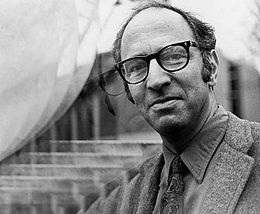
\includegraphics[width=0.15\textwidth]{figuras/kuhn.jpg}
		\\	% this spacer is needed to make the text on the right fit OK
	\end{wrapfigure}
	
	\NewsItem{A Estrutura das Revoluções Científicas}
	\NewsAuthor{Thomas Kuhn}
	{\small ``A transição de um paradigma em crise para um novo do qual pode surgir uma nova tradição de ciência normal está longe de ser um processo cumulativo obtido através de uma articulação do velho paradigma. É antes uma reconstrução da área de estudos a partir de novos princípios, reconstrução que altera algumas das generalizações teóricas mais elementares do paradigma, bem como muitos de seus métodos e aplicações. Durante o período de transição haverá uma grande coincidência (embora nunca completa) entre os problemas que podem ser resolvidos pelo antigo paradigma e os que podem ser resolvidos pelo novo. Haverá igualmente uma diferença decisiva no tocante aos modos de solucionar os problemas. [...] Outros que atentaram para esse aspecto do avanço científico enfatizaram sua semelhança com uma mudança na forma visual: as marcas no papel, que primeiramente foram vistas como um pássaro, são agora vistas como um antílope ou vice-versa. [...] A transição para um novo paradigma é uma revolução científica. [...] O que são revoluções científicas e qual a sua função no desenvolvimento científico? [...] Consideramos revoluções científicas aqueles episódios de desenvolvimento não-cumulativo, nos quais um paradigma mais antigo é total ou parcialmente substituído por um novo, incompatível com o anterior. Contudo, há muito mais a ser dito e uma parte essencial pode ser introduzida através de mais uma pergunta. Por que chamar de revolução uma mudança de paradigma? Face às grandes e essenciais diferenças que separam o desenvolvimento político do científico, que paralelismo poderá justificar a metáfora que encontra revoluções em ambos? [...] O estudo histórico da mudança de paradigmas revela características muito semelhantes a essas, ao longo da evolução da ciência. Tal como a escolha entre duas instituições políticas em competição, a escolha entre paradigmas em competição demonstra ser uma escolha entre modos incompatíveis de vida comunitária. Por ter esse caráter, ela não é e não pode ser determinada simplesmente pelos procedimentos de avaliação característicos da ciência normal, pois esses dependem parcialmente de um paradigma determinado e esse paradigma, por sua vez, está em questão. Quando os paradigmas participam - e devem fazê-lo - de um debate sobre a escolha de um paradigma, seu papel é necessariamente circular. [...] O historiador da ciência que examinar as pesquisas do passado a partir da perspectiva da historiografia contemporânea pode sentir-se tentado a proclamar que, quando mudam os paradigmas, muda com eles o próprio mundo. Guiados por um novo paradigma, os cientistas adotam novos instrumentos e orientam seu olhar em novas direções. E o que é ainda mais importante: durante as revoluções, os cientistas vêem coisas novas e diferentes quando, empregando instrumentos familiares, olham para os mesmos pontos já examinados anteriormente. É como se a comunidade profissional tivesse sido subitamente transportada para um novo planeta, onde objetos familiares são vistos sob uma luz diferente e a eles se apregam objetos desconhecidos. Certamente não ocorre nada semelhante: não há transplante geográfico; fora do laboratório os afazeres cotidianos em geral continuam como antes.''\par}
	\vspace{0.5cm}
	{\footnotesize \noindent \emph{*Thomas Kuhn foi um físico e filósofo da ciência estadunidense. Esse texto foi compilado da obra de Thomas Kuhn \emph{A Estrutura das Revoluções Científicas}, em edição na língua portuguesa publicada pela editora Perspectiva em 2011.}\par}
\end{minipage}
\end{center}
\vspace{0.5cm}
	\SepRule
\vspace{0.5cm}

%-----------------------------------
\newpage
\begin{multicols}{3}
% ------------------------------------------
% Texto dos editores sobre a Newsletter
% ------------------------------------------
\NewsItem{Sobre a Newsletter}
\NewsAuthor{Vasily Dokuchaev}
\begin{wrapfigure}{l}{0.15\textwidth}
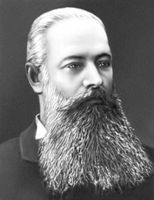
\includegraphics[width=0.15\textwidth]{figuras/dokuchaev.jpg}
\end{wrapfigure}
	{\small A ideia de criar uma Newsletter da Comissão de Pedometria da Sociedade Brasileira de Ciência do Solo (SBCS) surgiu durante a II reunião da Rede Brasileira de Pesquisa em Mapeamento Digital de Solos (RedeMDS), em outubro de 2012, na cidade de Florianópolis, Santa Catarina. Todos os pesquisadores presentes concordaram comigo que é preciso divulgar e desmistificar a pedometria e o mapeamento digital de solos (MDS) no Brasil. Nada melhor do que uma publicação periódica que permita aos pesquisadores brasileiros divulgar suas pesquisas pedométricas e, sobretudo, conhecerem uns aos outros (É por isso que eu sempre coloco a foto do autor do texto!). Isso é importante porque, assim como a própria pedometria, a maioria dos pesquisadores brasileiros dessa área também são bastante jovens, muitos dos quais ainda estão desenvolvendo seus estudos de mestrado e doutorado. Mas além disso, para que a pedometria cresça e seja reconhecida como disciplina da ciência do solo no Brasil, é preciso que mais pesquisadores queiram aventurar-se pelo mundo dos modelos matemáticos, sensores remotos e scripts de computador. É por isso que a Newsletter também está direcionada aos estudantes de graduação. Tento manter uma linguagem simples e direta, preferencialmente na voz ativa, para aproximar autor e leitor. Mas a melhor parte da Newsletter é que ela é distribuida gratuitamente. Foi por isso que a registrei sob a licença Creative Commons Atribuição-Compartilha Igual 3.0 Não Adaptada (CC-BY-SA).
	
	\begin{center}
		
\includegraphics[width=0.8\linewidth]{figuras/cc-by-sa.png}\\
		\caption{\footnotesize \textbf{Atribuição-Compartilha Igual 3.0 Não Adaptada.}}
	\end{center}	
		
	E como funciona a Newsletter? Em primeiro lugar, é importante dizer que a produção e distribuição da Newsletter é de responsabilidade da Comissão de Pedometria da Sociedade Brasileira de Ciência do Solo (SBCS). Entretanto, o conteúdo da Newsletter não representa o ponto de vista da Comissão de Pedometria ou da SBCS, mas sim de cada um dos autores dos textos publicados. Atualmente, Alessandro Samuel-Rosa, da Universidade Federal Rural do Rio de Janeiro, é o editor-chefe da Newsletter, e Jean Michel Moura-Bueno, da Universidade Federal de Santa Maria, é o editor assistente da Newsletter. Ambos são responsáveis por todo o processo de produção e distribuição da Newsletter sem qualquer custo administrativo, ou seja, trabalham voluntariamente.
	
	\begin{center}
		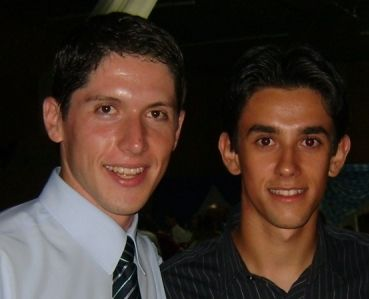
\includegraphics[width=0.8\linewidth]{figuras/editors.jpg}\\
		\caption{\footnotesize \textbf{Os editores voluntários.}}
	\end{center}	
	
	A ideia que eu tenho em mente é de que a Newsletter tenha uma edição produzida e distribuída gratuitamente a cada quatro meses, ou seja, nos meses de abril/maio, agosto/setembro e dezembro/janeiro. Qualquer pessoa interessada pode submeter um texto para publicação na Newsletter. Basta entrar em contato com um dos editores através dos endereços de e-mail disponíveis no final dessa edição (Não adianta tentar entrar em contato comigo porque eu não tenho nem telefone, nem endereço de e-mail e muito menos conta no Facebook!). A Newsletter está aberta aos mais diversos temas relacionados à pedometria, desde discussões sobre conceitos até a aplicação de sensores e modelos matemáticos, mas sempre usando uma linguagem simples, clara e direta. Mas já deixei claro aos editores que a Newsletter deve conter, sempre que possível, textos que abordem os seguintes temas: (a) explicitação de um conceito usado em pedometria, (b) entrevista de um pesquisador brasileiro, (c) a opinião de um pesquisador sobre um determinado tema relevante para a pedometria, (d) descrição de equipamentos e sensores remotos, (e) descrição de softwares e suas funcionalidades, e (f) eventos técnico-científicos da área.
	
	A elaboração dos textos publicados na Newsletter pode ser voluntária ou mediante convite feito pelos editores. Na presente edição, por exemplo, há um texto voluntário sobre o conceito de pedometria. Por outro lado, quatro pesquisadores foram convidados a discorrer sobre temas diversos como, por exemplo, o ensino de pedometria no Brasil, o uso de software livre, o desenvolvimento de pesquisas pedométricas na Antártica e o conteúdo pedométrico no XXXIV Congresso Brasileiro de Ciência do Solo (CBCS) (Na próxima edição, gostaria de ver a opinião dos leitores sobre as palestras que teremos em Floripa. É claro que eu estarei por lá! Afinal de contas, a abertura terá uma apresentação da Escola Bolshoi. Talvez até eu participe mostrando meus passos de ballet.). Acredito que os editores conseguiram elaborar uma boa primeira edição. Para a segunda edição já lhes solicitei a inclusão de um texto descrevendo as funcionalidades de algum pacote de análise de dados espaciais no R, software que muitos estão utilizando (Na verdade pedi isso aos editores porque quero aprender a usar esse tal de R! E eu que achava que o R era usado apenas pra indicar a camada de rocha na descrição do perfil de solo!). E, é claro, também quero ouvir dos leitores sugestões e críticas para melhorar a Newsletter (Ou melhor, reclamem com os editores!).\par}
	\vspace{0.5cm}
	{\footnotesize \noindent \emph{*Vasily Dokuchaev é o avatar dos editores. Qualquer semelhança com o naturalista russo Vasily Vasilievich Dokuchaev, considerado o pai da ciência do solo, é mera coincidência.}\par}
	
\newpage
% --------------------------------------------------------------------	
% Texto de Alessandro Samuel-Rosa sobre Pedometria
% --------------------------------------------------------------------	
\NewsItem{O que é Pedometria?}
\NewsAuthor{Alessandro Samuel-Rosa}
\begin{wrapfigure}{l}{0.15\textwidth}
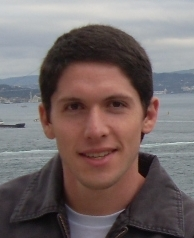
\includegraphics[width=0.15\textwidth]{figuras/alessandro.jpg}
\end{wrapfigure}
	{\small A pedometria é uma das mais novas disciplinas da ciência do solo. Utilizada desde os tempos de Jenny, mesmo que de maneira rudimentar, alcançou seu máximo desenvolvimento a partir do início da década de 1990. O termo pedometria, um neologismo derivado do grego \emph{pedos} (solo) e \emph{metron} (medida), foi proposto por Alex McBratney para identificar o estudo quantitativo da variação do solo no campo. Assim, o uso do termo pedometria é feito de maneira análoga a outros termos como econometria, biometria, psicometria, bibliometria, dendrometria, entre outras, assim como a mais antiga de todas, a geometria (Webster, 1994, McBratney et al., 2000).\par}
	
	{\small O termo cunhado por Alex McBratney tenta cobrir duas ideias principais (McBratney et al., 2000). A primeira delas está relacionada à parte da mensuração (\emph{metron}), sendo restrita aos métodos quantitativos matemáticos e estatísticos. A segunda delas está relacionada à parte do solo (\emph{pedos}), correspondendo à disciplina da ciência do solo chamada pedologia. Devido às diferentes interpretações que podem ser derivadas do termo cunhado por McBratney, diversas definições para o termo pedometria foram elaboradas, provavelmente tantas quanto o número de cientistas trabalhando nessa disciplina (Heuvelink, 2003). Vejamos algumas delas:\par}
	
	\begin{itemize}{\small
	 \item a aplicação de métodos matemáticos e estatísticos para a modelagem quantitativa do solo, com o objetivo de analisar sua distribuição, propriedades e comportamento;
	 \item a aplicação de métodos matemáticos e estatísticos para a descrição do solo;
	 \item o desenvolvimento e aplicação de métodos estatísticos e matemáticos aplicáveis a problemas de análise de dados em ciência do solo;
	 \item ciência do solo sob incerteza;
	 \item a aplicação de métodos matemáticos e estatísticos para o estudo do solo;
	 \item medidas do solo;
	 \item o uso de métodos quantitativos para o estudo da distribuição e gênese do solo, e como um recurso sustentável;
	 \item matemática do solo;
	 \item estudo da variação das propriedades do solo;
	 \item o estudo e manipulação de dados experimentais em ciência do solo;
	 \item ...
	\par}
	\end{itemize}
	
	{\small Mesmo havendo uma miríade de conceitos e, em alguns casos, discordância entre os cientistas, a pedometria evoluiu consideravelmente nas duas últimas décadas. Isso significa que é perfeitamente possível continuar trabalhando sem a elaboração de um conceito universal. Entretanto, existem dois motivos importantes para a elaboração de um conceito que represente a visão geral de uma comunidade científica em relação ao seu campo de atuação. O primeiro deles está relacionado à necessidade de comunicação com cientistas de outras áreas do conhecimento, sejam eles da ciência do solo ou não (Heuvelink, 2003). A contextualização constitui uma parte fundamental do preparo do terreno para a utilização eficiente da linguagem (Wittgenstein, 1999). A própria divulgação da pedometria como nova disciplina da ciência do solo, assim como sua aceitação pela comunidade científica, exige uma “delimitação” conceitual, mesmo que isso seja operacionalmente impossível (McBratney et al., 2000). O segundo motivo está relacionado à necessidade de comunicação com os jovens cientistas, os quais ainda estão em processo de escolha de sua área de atuação e formação de seus próprios conceitos. Como resultado dessas necessidades, a seguinte definição de pedometria foi elaborada pela Comissão de Pedometria da União Internacional de Ciência do Solo (IUSS) (Heuvelink, 2003):\par}
	
	\begin{center}
	{\small \textbf{\emph{Aplicação de métodos matemáticos e estatísticos para o estudo da distribuição e gênese do solo.}}\par} 
	\end{center}
	
	{\small A utilização da expressão “\emph{métodos matemáticos e estatísticos}” carrega, implícita, a noção de que os estudos são de caráter mais quantitativo do que qualitativo (Burrough et al., 1994). No que diz respeito à “\emph{gênese do solo}”, o objetivo é explicitar, numericamente, a relação entre os fatores de formação do solo, expressos na forma de variáveis ambientais obtidas através de sensores remotos, modelos digitais de elevação, mapas geológicos, etc, com os atributos apresentados pelo solo. Por fim, a “\emph{distribuição do solo}” é abordada nos três “meios” em que o solo apresenta potencial de variação: o espaço geográfico, o tempo e o espaço de atributos. As principais ferramentas utilizadas para alcançar os objetivos da pedometria são a geoestatística, a estatística tradicional (modelos lineares generalizados, redes neurais, árvores de decisão e regressão, etc), e a combinação das duas, que dá origem ao que tem sido chamado de métodos híbridos.\par}
	
	{\small Na prática, a pedometria envolve uma série de estudos em ciência do solo, havendo sobreposição com muitas das demais disciplinas e áreas do conhecimento. Um dos principais exemplos de aplicação da pedometria é o mapeamento digital do solo, o qual pode se utilizar das chamadas funções de pedotransferência, outra ferramenta desenvolvida a partir da utilização dos métodos pedométricos. Nesse caso, a pedometria se sobrepõe, por exemplo, à pedologia (mapeamento do solo) e à quimiometria (do inglês, \emph{chemometrics}). Além disso, a pedometria trata da aplicação de sensores remotos para a obtenção de informações do solo, assim como o desenvolvimento de sistemas de informação pedológica, plataformas de bancos de dados, entre outras ferramentas relacionadas à informática e eletrônica. Soma-se ainda as possibilidades de aplicação em áreas como a biologia e microbiologia do solo, física do solo, entre outras.\par}
	\vspace{0.5cm}
	\noindent \textbf{Referências}\\
	\\
	{\footnotesize \noindent Burrough, P.A.; Bouma, J. & Yates, S.R. The state of the art in pedometrics. Geoderma, 62:311-326, 1994.\par}
	{\footnotesize \noindent Heuvelink, G.B.M. The definition of pedometrics. Pedometron, 15:11-12, 2003.\par}
	{\footnotesize \noindent McBratney, A.B.; Odeh, I.O.; Bishop, T.F.; Dunbar, M.S. & Shatar, T.M. An overview of pedometric techniques for use in soil survey. Geoderma, 97:293-327, 2000.\par}
	{\footnotesize \noindent Webster, R. The development of pedometrics. Geoderma, 62:1-15, 1994.\par}
	{\footnotesize \noindent Wittgenstein, L. Investigações filosóficas. São Paulo, Nova Cultural, 1999. 207p.\par}
	\vspace{0.5cm}
	{\footnotesize \noindent \emph{*Alessandro Samuel-Rosa é doutorando do Curso de Pós-graduação em Agronomia-Ciência do Solo da UFRRJ e mantenedor do site soil-scientist.net.}\par}

\newpage
% --------------------------------------------------------------------
% Entrevista com Alexandre ten Caten feita por Jean Michel Moura-Bueno
% --------------------------------------------------------------------
\NewsItem{Entrevista com o Cientista}
\NewsAuthor{Jean M. Moura-Bueno}
\begin{wrapfigure}{l}{0.15\textwidth}
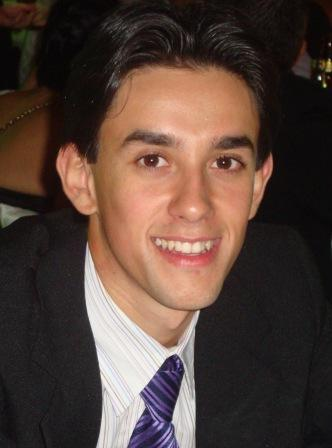
\includegraphics[width=0.15\textwidth]{figuras/jean.jpg}
\end{wrapfigure}
	{\small A Ciência do Solo é uma área do conhecimento que contempla várias disciplinas, as quais contribuem para o avanço na  aquisição de informações a respeito do solo. Uma dessas disciplinas é a Pedometria. Para discorrer mais sobre essa disciplina, suas potencialidades, dificuldades e perspectivas futuras no Brasil, entrevistamos o Dr. Alexandre ten Caten, professor do curso de Ciências Rurais da Universidade Federal de Santa Catarina, Campus Curitibanos. Sua formação pós ensino médio foi realizada na Universidade Federal de Santa Maria (UFSM), contemplando formação técnica em Geoprocessamento, graduação em Agronomia, e mestrado e doutorado em Ciência do Solo na área de mapeamento digital do solo (MDS). Publicou recentemente uma revisão bibliográfica discorrendo sobre o MDS no Brasil, com ênfase nas abordagens das pesquisas realizadas sobre o MDS (ten Caten et al., 2012).\par}
	
	\begin{center}
			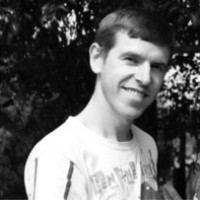
\includegraphics[width=0.6\linewidth]{figuras/ten-caten2}\\
			\caption{\footnotesize \textbf{Dr. Alexandre ten Caten.}}
	 \end{center}
	
	\begin{itemize*}
	{\small
	 \item \textbf{O que levou você a se interessar e estudar sobre o MDS e em especial temas relacionados a pedometria?}
	 Durante a graduação uma área que me despertou grande interesse foram os temas relacionados à Geomática. Ao ingressar para o mestrado em Ciência do Solo eu queria utilizar as ferramentas ligadas às geotecnologias no mapeamento de solos. Eu já era sabedor das potencialidades do Sensoriamento Remoto e da Aerofotogramentria para os levantamentos de solos, no entanto, não tinha total clareza de como desenvolveria meu projeto de mestrado. Em uma ocasião, enquanto fazia uma busca por artigos, me deparei com o material publicado por McBratney e colaboradores \emph{On Digital Soil Mapping}, devo dizer que ter encontrado este material foi um divisor de águas, não só para meu projeto de mestrado e doutorado, como também posteriormente, no meu interesse pela pesquisa integrando estatística, ciência do solo e geoinformação.
	 \item \textbf{Quais são os projetos de pesquisa que você está desenvolvendo?}
	 Nossa principal linha de pesquisa busca investigar as potencialidades do sensoriamento proximal para a determinação de propriedades do solo.
	 \item \textbf{O que você acha do cenário atual da pedometria no Brasil?}
	 A área tem conquistado espaço na pesquisa em ciência do solo do país. Nos eventos científicos, como o Congresso Brasileiro de Ciência do Solo, são crescentes os trabalhos e palestras apresentados neste tópico. A reunião de um grupo de pesquisadores na \emph{RedeMDS} tem possibilitado a troca de experiências e a capacitação dos pesquisadores neste tópico.
	 
	 \begin{center}
			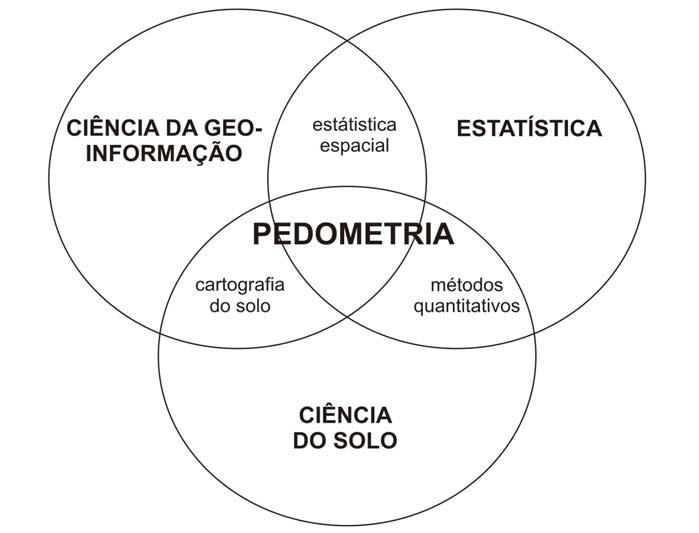
\includegraphics[width=1\linewidth]{figuras/fig-ten-caten}
			\caption{\footnotesize \textbf{A Pedometria como uma ciência interdisciplinar.\\Fonte: ten Caten (2008).}}
	 \end{center}
	 
	 \item \textbf{Qual a sua opinião a respeito da pedometria como uma disciplina nos cursos de Graduação e Pós-Graduação em Ciência do Solo no Brasil?}
	 A formação em nível de graduação tem de possibilitar uma forte base aos graduandos em disciplinas como estatística, geologia, ciência do solo, informática e geoprocessamento. A pedometria irá conquistar seu espaço em nível de pós-graduação na medida em que for mais conhecida e explorada. Isso, com certeza, é um processo natural, e que também ocorreu com outras áreas do conhecimento como a nanotecnologia e a bioinformática. A pedometria é uma área integradora de conhecimentos, e essa possibilidade de investigação científica tem despertado interesse dos pesquisadores. Com dissertações e teses aplicando os conhecimentos relacionados à pedometria, será cada vez maior o número de pesquisadores capacitados para oferecer disciplinas com algum grau de relação com a pedometria.
	 \item \textbf{Quais as perspectivas futuras da pedometria no Brasil?}
	 Promissoras. As pesquisas, assim como as publicações dos resultados, estão em uma crescente. A possibilidade de predizer classes e propriedades do solo já está cientificamente comprovada. A pesquisa em pedometria precisa avançar agora para a geração da informação espacial em solos por demanda. Os mapas de solos são tradicionalmente gerados sem uma aplicação determinada \emph{a priori}, o que torna a informação gerada generalista. Com a possibilidade de produzir um levantamento de solos, seja de classe ou propriedades, a partir de uma necessidade específica, haverá um melhor ajuste entre amostragem, escala e exatidão da informação produzida. Contudo, para que este passo seja dado, os possíveis \emph{clientes} da informação do solo devem ter o conhecimento da importância do solo para seus projetos. Isso nos remete novamente ao papel da Sociedade Brasileira de Ciência do Solo em fomentar as discussões da relevância do solo para a sociedade.
	 \item \textbf{Quais as dificuldades e desafios dos jovens pesquisadores em trabalhar com a pedometria?}
	 Integrar conhecimentos relacionados a distintas disciplinas como ciência do solo, estatística, informática e geotecnologias.
	 \item \textbf{Você acha a pedometria uma ferramenta promissora para ser utilizada na obtenção de informações de qualidade sobre solos?}
	 A pedometria pode ser empregada em várias aplicações. Não somente avaliando a qualidade do solo, mas também, para gerar informações a respeito do próprio solo e das ameaças a ele, e isso em distintas escalas.
	 \par}
	\end{itemize*}
	
	\vspace{0.5cm}
	
	\noindent \textbf{Referências}\\
	\\
	{\footnotesize \noindent ten Caten, A. Application of principal components and multiple logistic regression in a geographical information system for prediction and digital soil mapping. Universidade Federal de Santa Maria, Santa Maria, 2008, 130p. (Dissertação de mestrado)\par}
	{\footnotesize \noindent ten Caten, A.; Dalmolin, R.S.D.; Mendonça-Santos, M.L.; Giasson, E. Mapeamento digital de classes de solos: características da abordagem brasileira. Ciência Rural, v.42, p.1989-1997, 2012.\par}
	\vspace{0.5cm}
	{\footnotesize \noindent \emph{*Jean Michel Moura-Bueno é mestrando do Programa de Pós-graduação em Ciência do Solo da UFSM.}\par}
\newpage
% -------------------------------------------------------
% Texto de Gustavo de Mattos Vasques sobre software livre
% -------------------------------------------------------
\NewsItem{Uma nota sobre software livre}
\NewsAuthor{Gustavo M. Vasques}
\begin{wrapfigure}{l}{0.15\textwidth}
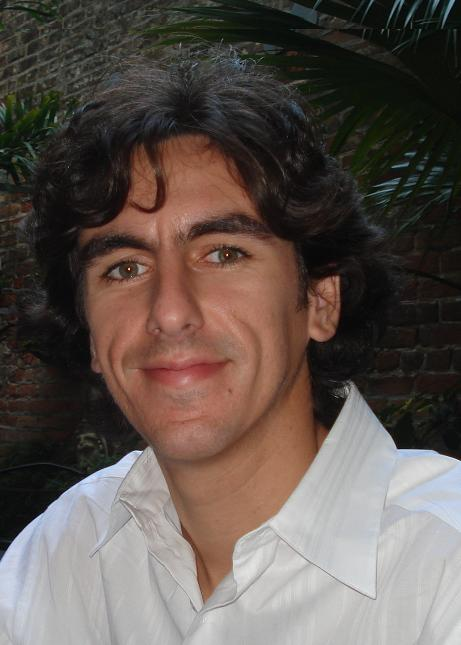
\includegraphics[width=0.15\textwidth]{figuras/gustavo.jpg}
\end{wrapfigure}
	{\small Como qualquer ramo da ciência, a ciência do solo mantém-se através de programas e projetos de pesquisa, ensino e extensão, que visam a solucionar desde problemas locais até problemas de interesse global. Como os recursos financeiros para custear tais projetos são limitados, existe uma competição entre grupos de pesquisa por fatias desses recursos. Nesse ponto, qualquer ajuste que dê vantagem competitiva ao grupo de pesquisa é bem vindo, notadamente a eficiência no uso dos recursos financeiros, humanos e do tempo.
	
	Dentro dessa perspectiva, há uma tendência no meio científico de adoção de softwares livres que permitam realizar, de maneira barata e eficiente, desde tarefas básicas de informática, como elaboração de textos, preparação de apresentações e organização de arquivos, até a análise de dados e produção e publicação de resultados de pesquisa.
	
	\begin{center}
		
\includegraphics[width=0.8\linewidth]{figuras/linux}\\
		\caption{\footnotesize \textbf{Tux, o mascote do SO Linux.\\Fonte: Wikipedia.}}
	\end{center}
		
	Interessantemente, essa tendência vem contrapor o caráter competitivo da produção científica, pois, ao contrário, se firma como um movimento de colaboração para o desenvolvimento de soluções de problemas de interesse coletivo. Um exemplo clássico dessa tendência é o sistema operacional Linux, cujas diversas versões se adéquam às necessidades específicas dos usuários, que, conjuntamente, auxiliam e retroalimentam o desenvolvimento do sistema, o tornando cada vez mais robusto, universal e versátil.
	
	Outro exemplo clássico é o software estatístico R. Na verdade, o R é uma linguagem de programação criada para dar suporte à manipulação e análise estatística de dados. Atualmente, o R é o “braço direito” e a “menininha dos olhos” de muitos professores, pesquisadores e estudantes, que praticamente já substituíram todos os outros softwares estatísticos por ele. Por outro lado, é ainda “sonho de consumo” de tantos outros que desejam migrar para ele (e para outros softwares livres).
	
	\begin{center}
		
\includegraphics[width=0.8\linewidth]{figuras/grass-gis}\\
		\caption{\footnotesize \textbf{O logotipo do GRASS GIS.\\Fonte: Wikipedia.}}
	\end{center}
		
	Bem, “sonho de consumo” com certeza não é o termo mais apropriado, pois – assim como o Linux, o GRASS, o LibreOffice, algumas ferramentas do Google e até o Microsoft Internet Explorer – o R é gratuito. Aqui mereceria uma discussão mais detalhada sobre as diferenças de liberdade que existem entre softwares ditos “livres”, mas deixo essa busca ao leitor (pode começar pela Wikipedia, que também é livre), pois prefiro dedicar essas últimas linhas àqueles que estão iniciando no mundo do software livre, como eu, ou que querem iniciar-se.
	
	Um amigo meu conta uma história interessante sobre um senhor que começou tarde a sua carreira, mas com perseverança e esforço, dedicando o seu tempo para aprender novas coisas e implementar novos projetos, tornou-se muito bem sucedido. Sua história é para reforçar o jargão e convencer as pessoas de que “nunca é tarde para começar”.
	
	\begin{center}
		
\includegraphics[width=0.8\linewidth]{figuras/Rlogo}\\
		\caption{\footnotesize \textbf{O logotipo do Projeto R.\\Fonte: Wikipedia}}
	\end{center}
		
	Eu encaro esse processo de migração para software livre e de interação com esse tipo de software como uma relação de amor e ódio, que requer esforço, dedicação e perseverança (bem, como tudo ou quase tudo na vida). Por exemplo, se acostumar a escrever linhas de comando ao invés de apertar botão, para muitos, é difícil. Aí é necessário prática mesmo, não tem jeito. Para aqueles com esse tipo de dificuldade existem muitos softwares livres que apresentam interfaces gráficas amigáveis e ainda permitem “apertar botão”, inclusive algumas extensões do próprio R.

	\begin{center}
		
\includegraphics[width=0.8\linewidth]{figuras/libreoffice}\\
		\caption{\footnotesize \textbf{O logotipo do LibreOffice.\\Fonte: Wikipedia}}
	\end{center}
	
	Entretanto, a decisão de adoção de um primeiro software livre pode ser um passo inicial importantíssimo do que pode ser uma relação próspera e duradoura. No R, uma relação como essa permitiria, por exemplo, rodar um tipo de análise em lote (batch) com diferentes dados de entrada sem precisar apertar botões para “carregar os dados”, “selecionar o tipo de análise”, “selecionar as opções de análise”, “selecionar as variáveis”, “escolher as informações de saída”, etc., etc., etc., toda vez e para cada dado de entrada. Permitiria ainda trocar scripts com outros usuários, desenvolver soluções customizadas para problemas específicos, buscar ajuda em fóruns, tutoriais e inúmeros materiais gratuitos e, é claro, economizar muuuito dinheiro.\par}

	\vspace{0.5cm}
	
	{\noindent \footnotesize \emph{*Gustavo de Mattos Vasques é pesquisador da Embrapa Solos e iniciante nos softwares livres SAGA GIS e R.}\par}

\newpage
% ---------------------------------------------------------------------------------------
% Texto sobre pedometria no continente gelado, preparado por André Geraldo de Lima Moraes
% ---------------------------------------------------------------------------------------
\NewsItem{A Pedometria na Antártica}
\NewsAuthor{André G. L. Moraes}
\begin{wrapfigure}{l}{0.15\textwidth}
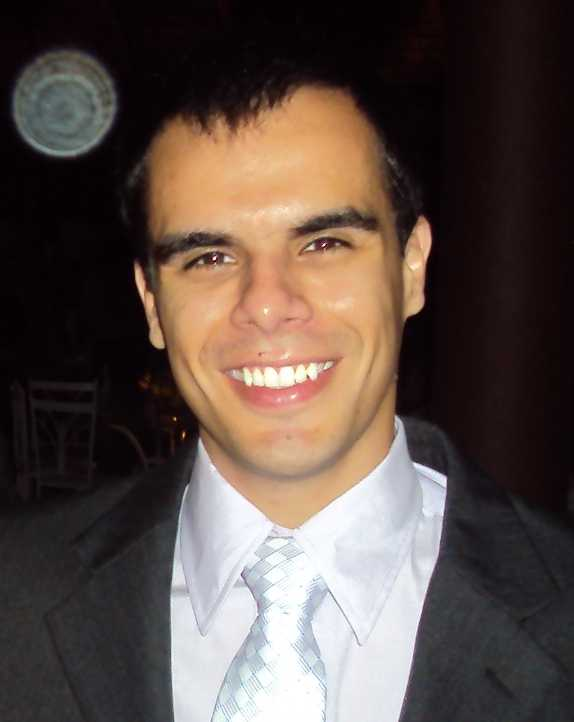
\includegraphics[width=0.15\textwidth]{figuras/andre.jpg}
\end{wrapfigure}
	{\small Eu sou mais um iniciante na área de Mapeamento Digital de Solos. E meu primeiro contato com esta área de estudo foi em janeiro de 2012, quando fui até o continente antártico realizar a coleta das amostras que fariam parte da pesquisa que desenvolverei no mestrado.
	
	O objetivo dos meus estudos é usar técnicas de Mapeamento Digital de Solos para mapear regiões periglaciares, ou seja, áreas livres de gelo (no verão) onde há processos pedogenéticos ativos, mesmo que em taxas muito lentas, devido às baixas temperaturas. A nossa área de estudo fica na península Keller - ilha Rei George, Antártica Marítima, onde se encontra a estação antártica brasileira (EACF).
	
	\begin{center}
		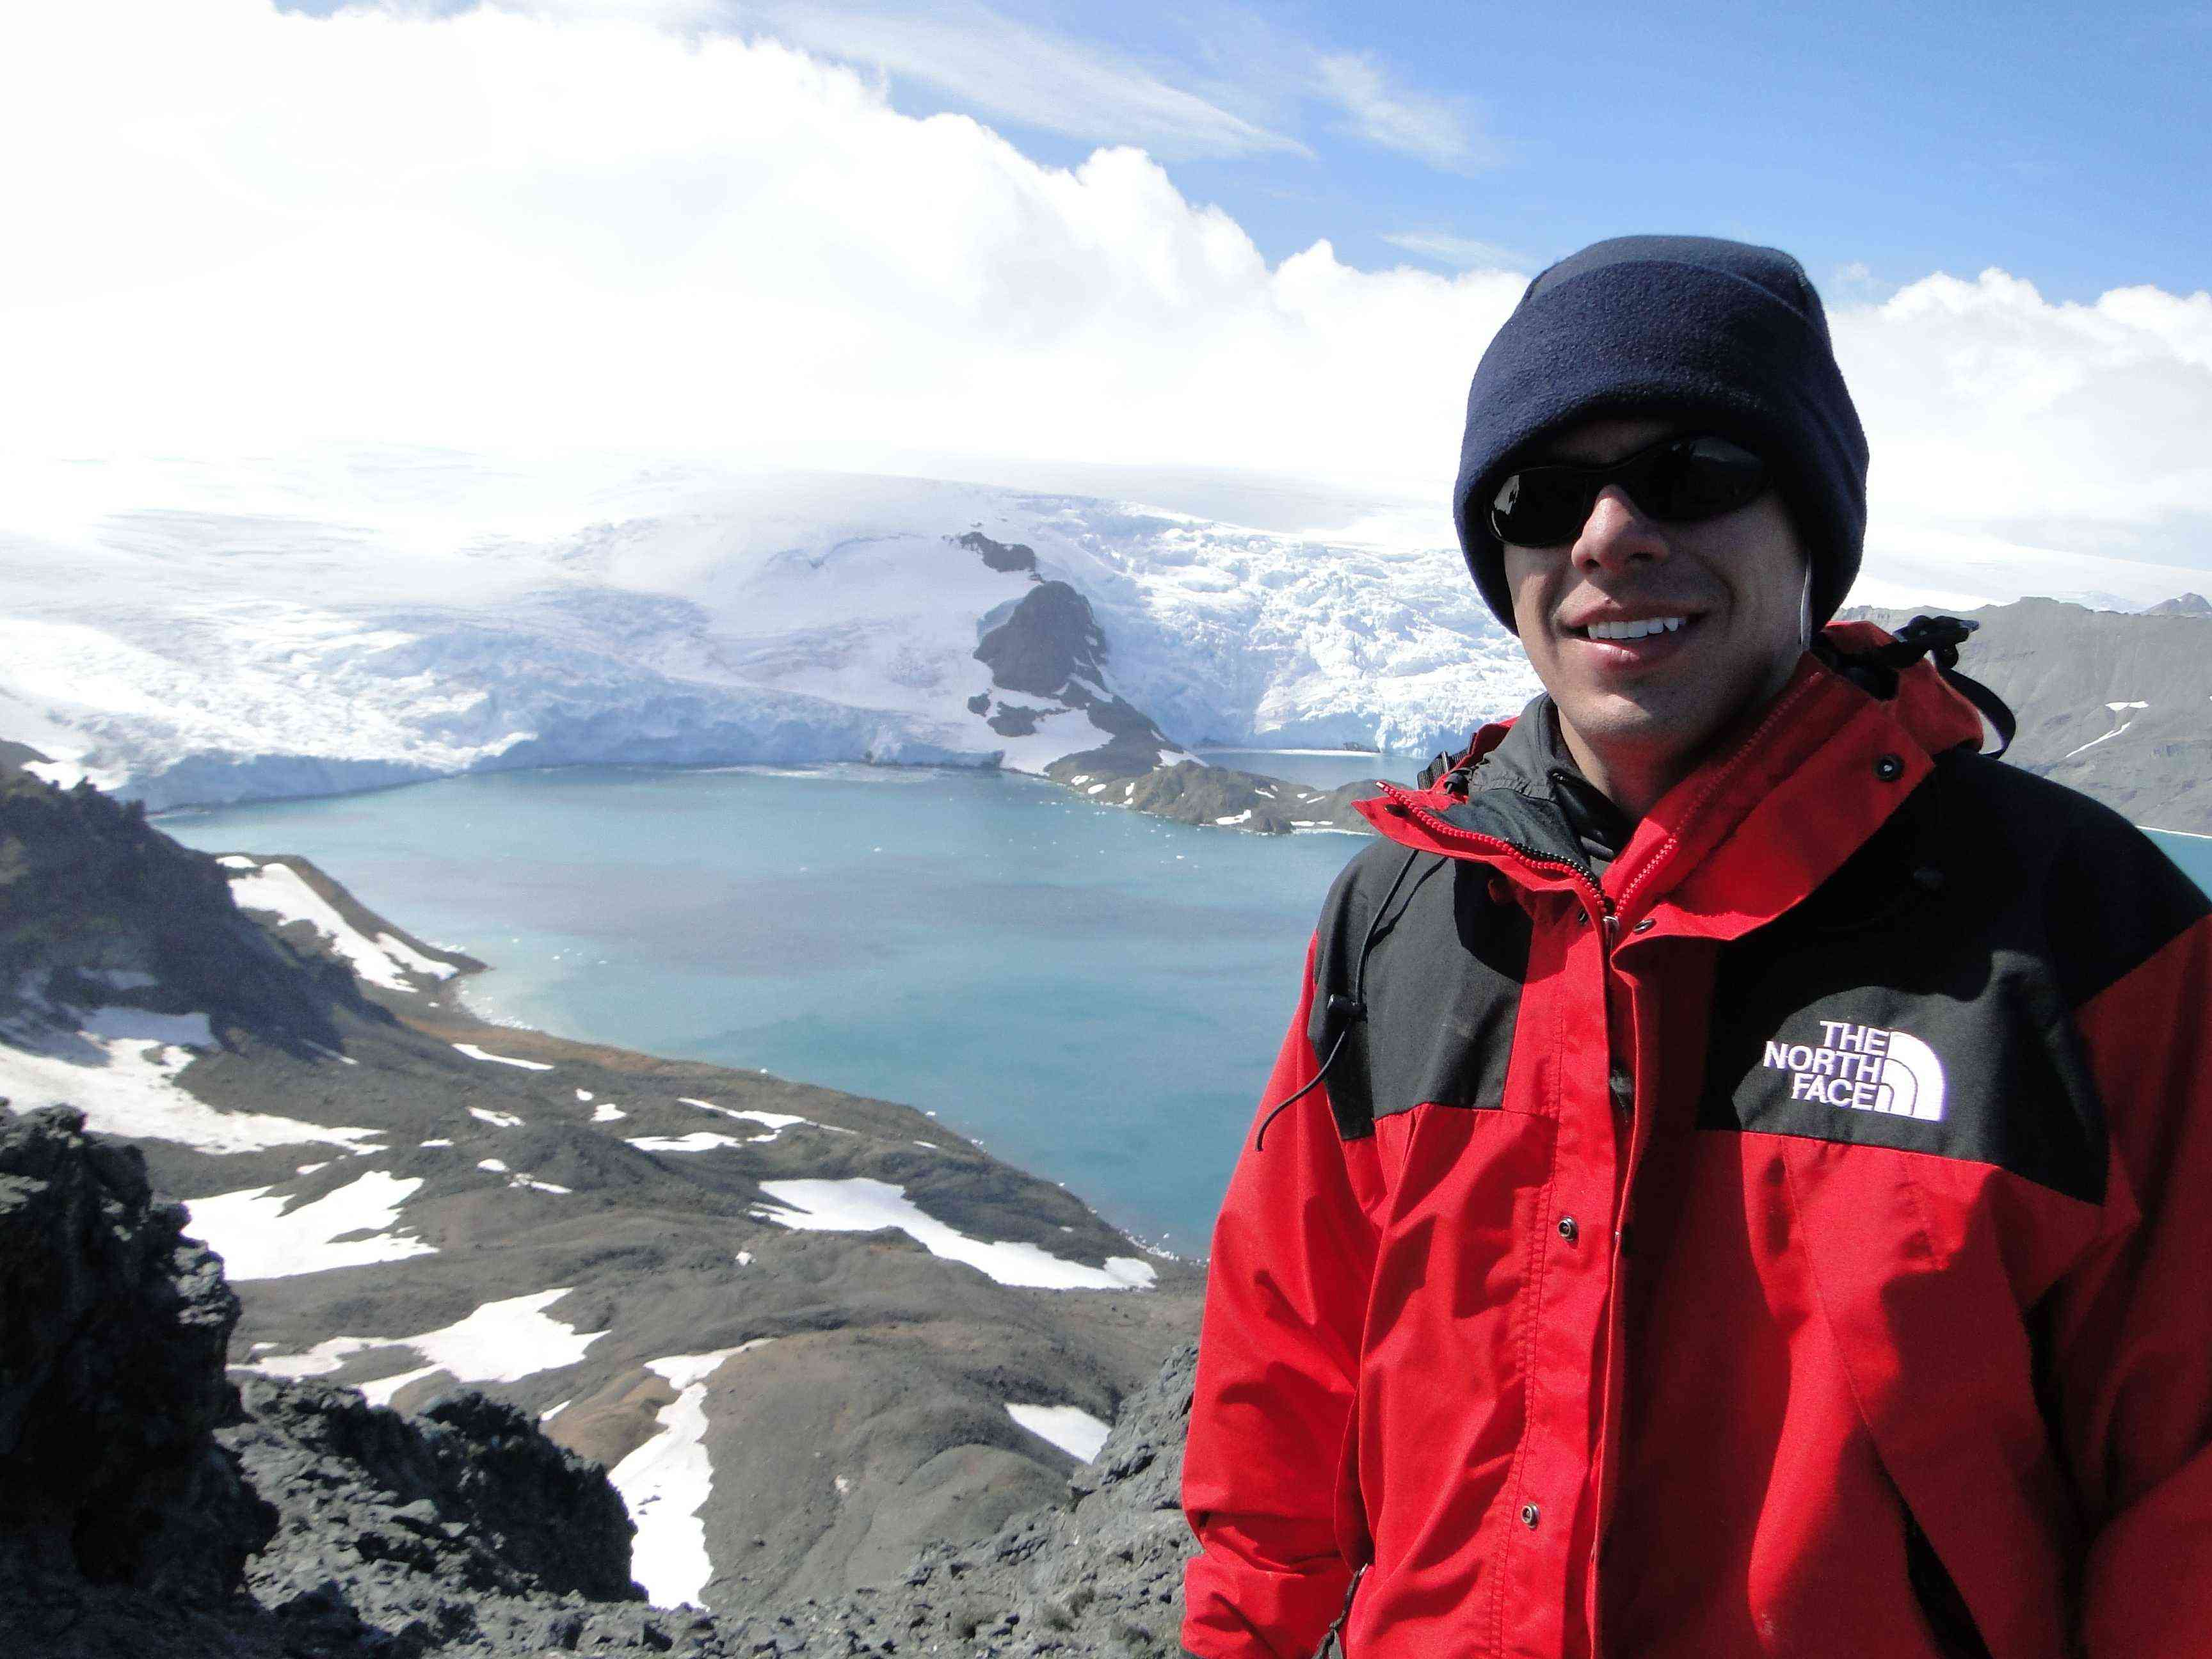
\includegraphics[width=0.8\linewidth]{figuras/andre2}\\
		\caption{\footnotesize \textbf{O continente gelado.}}
	\end{center}
	
	Mas ir para o continente gelado não é tarefa fácil. E devido aos vários perigos incluídos nesta missão, todos os pesquisadores que se propõem a ir para lá devem passar por um treinamento. Eu fiz o meu treinamento Pré-Antartico em agosto de 2011. O treinamento foi oferecido pelo Programa Antártico Brasileiro (PROANTAR) e pela Marinha do Brasil, auxiliados pelos alpinistas do Clube Alpino Paulista (CAP). O treinamento para ir para o continente mais frio de todos foi feita na Restinga da Maranbaia, em uma base da Marinha em meio a um paraíso tropical. Em sete dias de treinamento, os pesquisadores são apresentados aos perigos e dificuldades que enfrentarão no continente gelado e também instruídos para superar estas adversidades.
	
	\begin{center}
		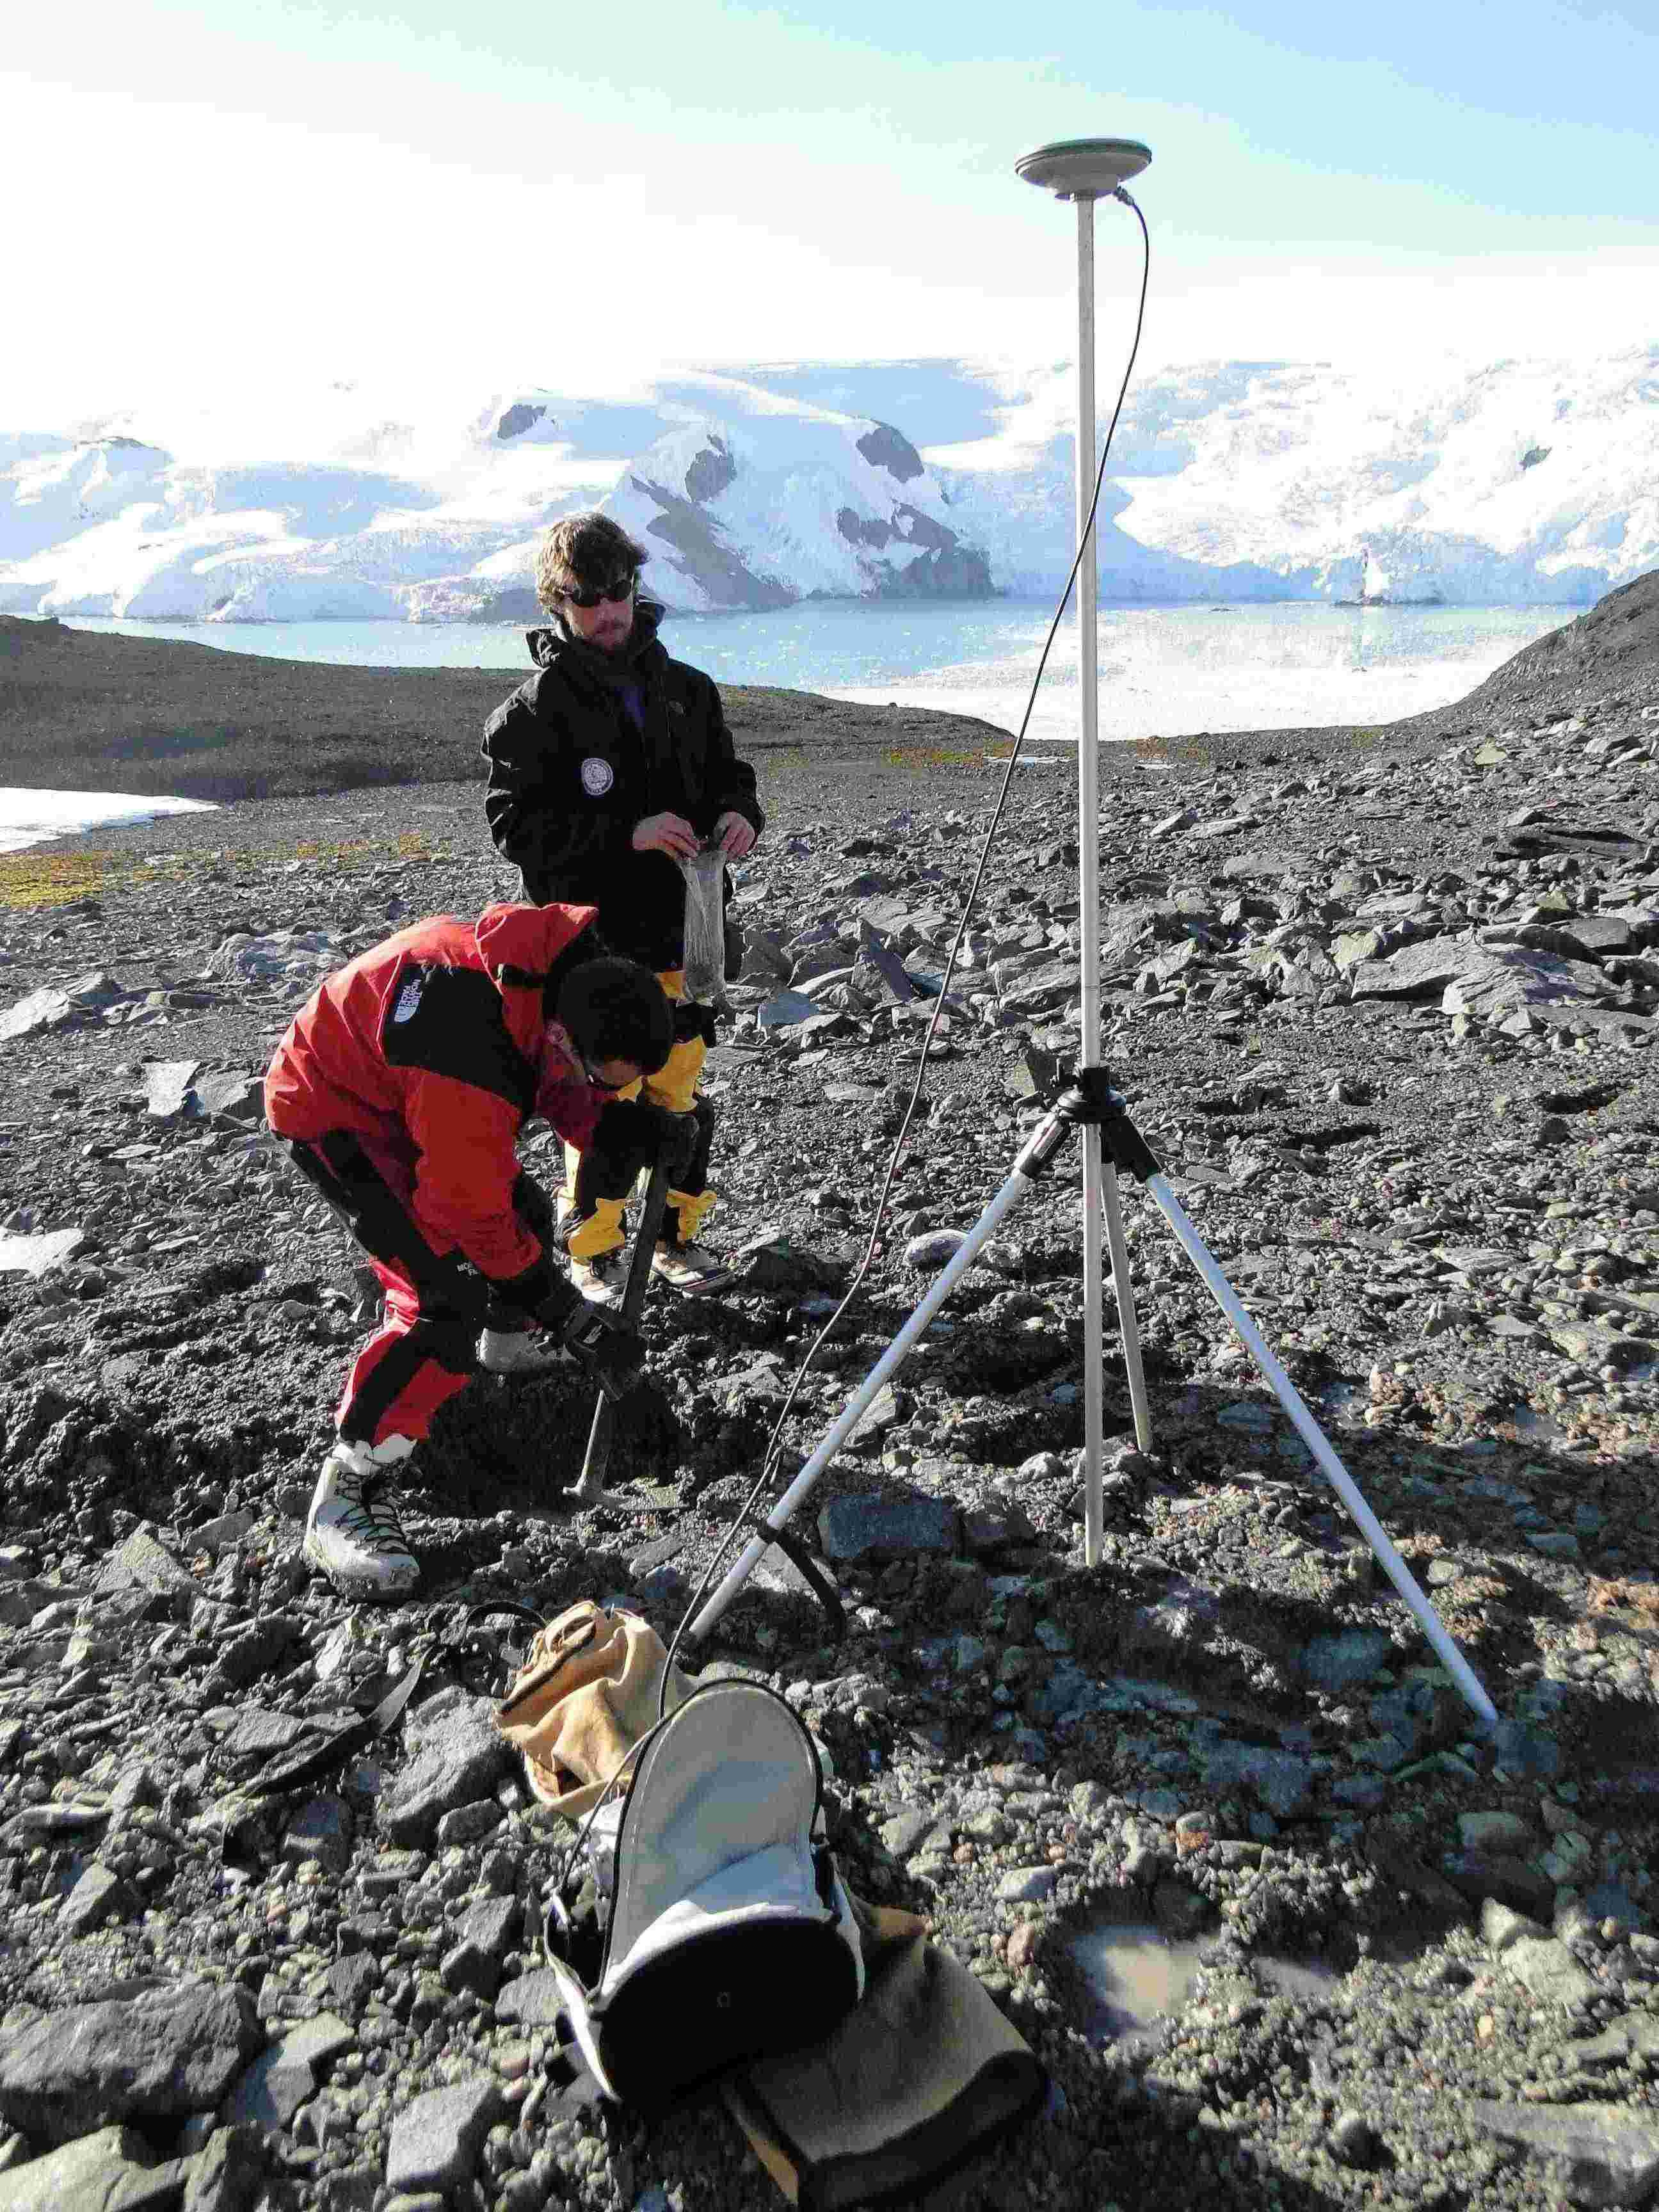
\includegraphics[width=0.8\linewidth]{figuras/andre4}\\
		\caption{\footnotesize \textbf{Amostragem de solo.}}
	\end{center}

	Em janeiro de 2012 eu pude ver e sentir as adversidades deste local de pesquisa e citarei agora alguns dos problemas que eu e minha equipe encontramos. Os pontos seriam coletados em forma de uma malha regular que cobriria toda a península que possui aproximadamente 500 ha. O nosso objetivo era de coletar 53 pontos, porém conseguimos coletar apenas 47. Seis dos pontos caíram em locais onde o acesso era impossível, ou estavam sobre glaciares ou neveiros. E muitos pontos foram coletados em áreas próximas de onde seriam realmente coletados, se tivéssemos coletado seguindo a grade regular. Outra limitação que tivemos foi em relação ao número de pontos coletados, pois as condições de trabalho na Antártica são muito complicadas (terreno muito movimentado e pedregoso, peso das amostras e equipamentos que são carregados em mochilas além do clima frio e algumas vezes chuvoso). Outro fator que nos deixou receosos foi a heterogeneidade do terreno, que além de ser muito movimentado, apresenta influência de vários materiais de origem diferentes.
	
	\begin{center}
		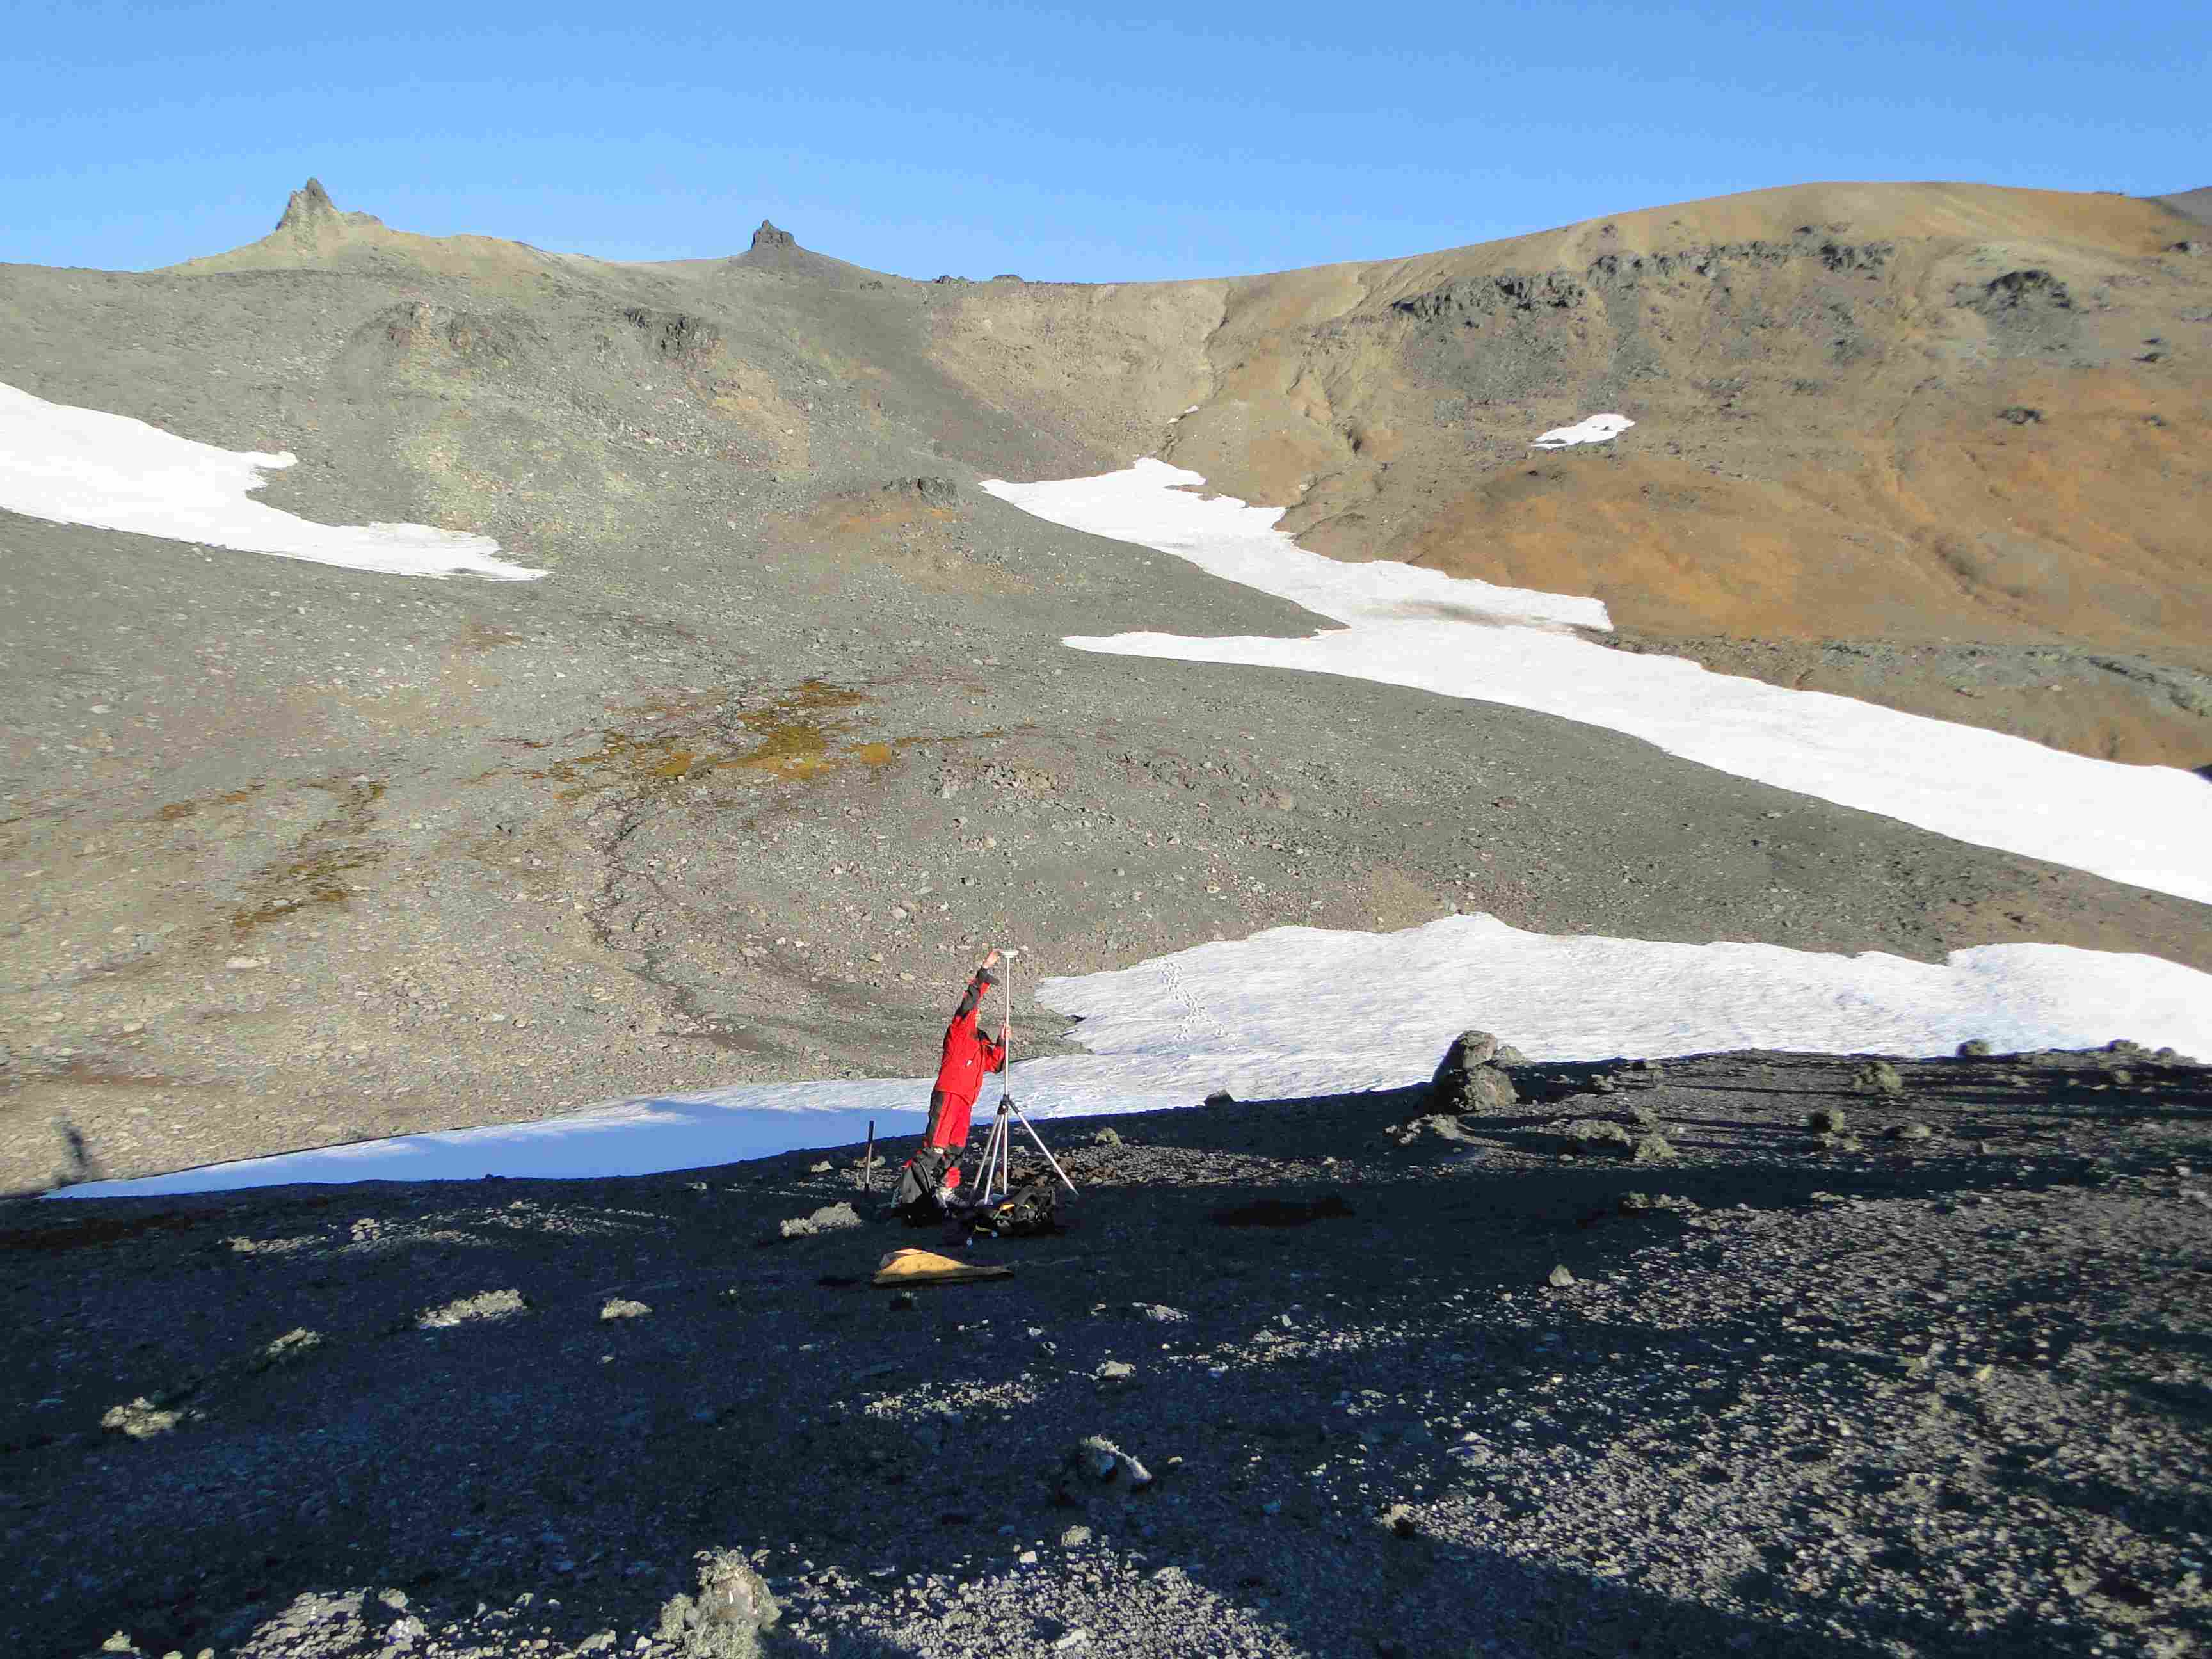
\includegraphics[width=0.8\linewidth]{figuras/andre5}\\
		\caption{\footnotesize \textbf{A paisagem antártica.}}
	\end{center}

	Nosso trabalho com MDS nesta área esta apenas na metade, e agora que estamos começando a gerar os modelos. Para tanto estamos utilizando software R que está se mostrando muito promissor para este tipo de análise. Também utilizamos do ArcGis 10.0 para gerar o MDE e o SagaGis para gerar os atributos de terreno que serão utilizados como covariáveis.
	
	\begin{center}
		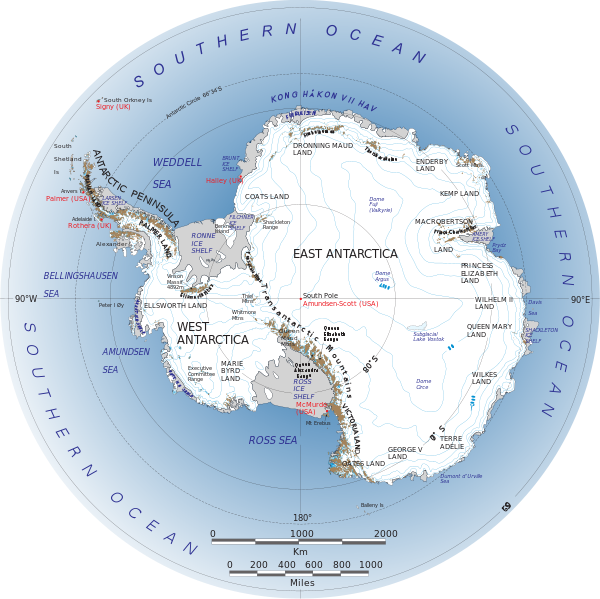
\includegraphics[width=0.8\linewidth]{figuras/antartica}\\
		\caption{\footnotesize \textbf{Mapa da antártica.\\Fonte: Wikipedia.}}
	\end{center}
	
	Nossa equipe está confiante, e resultados preliminares indicam que este tipo de técnica de mapeamento poderá ser utilizado com sucesso nesta região. Nossa equipe engloba discentes e docentes da UFRRJ (Macio R. Francelino e Marcos G. Pereira) e UFV (Carlos Ernesto Schaefer) fazendo parte do grupo TERRANTAR e INCT-CRIOSFERA, além de contribuições de membros da EMBRAPA-SOLOS (Waldir de  Carvalho Junior). Este trabalho não seria possível sem o apoio do Programa Antártico Brasileiro (PROANTAR), da Marinha do Brasil e do CNPq.\par}
	
	\vspace{0.5cm}
	
	{\noindent \footnotesize \emph{*André Geraldo de Lima Moraes é mestrando do Curso de Pós-graduação em Agronomia-Ciência do Solo da UFRRJ.}\par}

\newpage
% ----------------------------------------------------------------------------
% Texto de Ricardo Simão Diniz Dalmolin sobre o ensino de pedometria no Brasil
% ----------------------------------------------------------------------------
\NewsItem{A Pedologia, o Mapeamento Digital de Solo e as novas tecnologias de capacitação}
\NewsAuthor{Ricardo S. D. Dalmolin}
\begin{wrapfigure}{l}{0.15\textwidth}
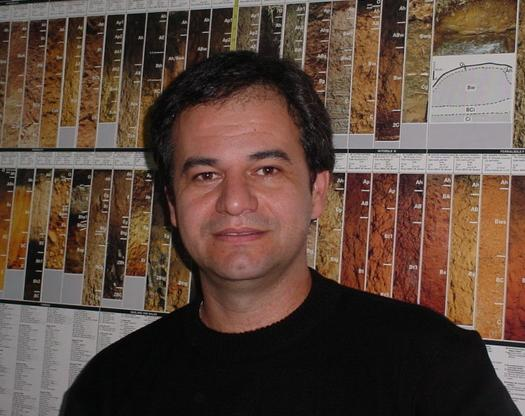
\includegraphics[width=0.15\textwidth]{figuras/dalmolin.jpg}
\end{wrapfigure}
	{\small O mapeamento digital de solos (MDS) é um campo de pesquisa relativamente recente e que tem crescido de maneira significativa em publicações internacionais. No Brasil, mesmo que a passos lentos, há um significativo aumento no número de artigos publicados e grupos de pesquisas envolvidos com MDS. Diria que, esse novo campo de pesquisa chegou para auxiliar, melhorar, incrementar ou qualquer outro adjetivo que soa como positivo no sentido de mapear, identificar, modelar, comparar informações a respeito de classes e/ou atributos do solo. Enfrentamos hoje, no meu entendimento, uma nova era da pedologia. O já discutido tópico que a pedologia está em declínio (veja Basher (1997), Dalmolin (1999) e Ker (1999)) pode ser substituído por essa nova afirmação: a pedologia estava em declínio ou, para ser mais otimista, “a pedologia está em ascensão”, e talvez o “culpado” seja o MDS.
		
	\begin{center}
		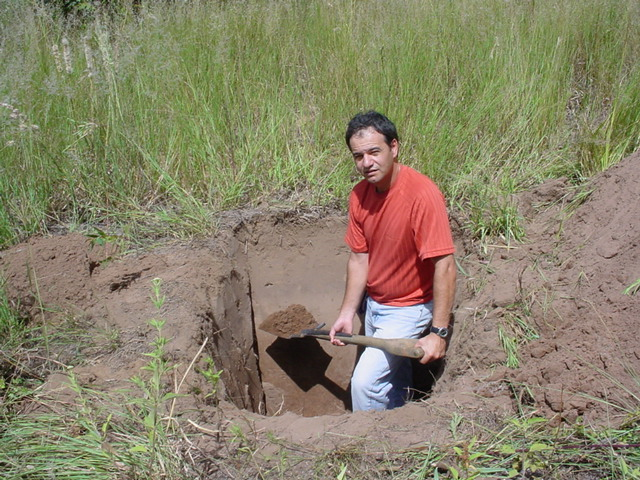
\includegraphics[width=0.8\linewidth]{figuras/pedo-dalmolin}\\
		\caption{\footnotesize \textbf{Um pedólogo da geração intermediária.}}
	\end{center}
	
	Com a entrada de novos pesquisadores, ou novos pedólogos, impulsionados principalmente pelo avanço tecnológico em termos de equipamentos, sensores, softwares (e um grande destaque aos softwares livres e de código aberto), além de técnicas e informações estatísticas, é que defendo a opinião de que entramos em uma nova era da pedologia. Sou grato, como pedólogo da geração intermediária (se classificarmos os pedólogos, considerando idade e tempo de atuação, como novos, intermediários e avançados), em assistir essa transição na qual os novos pedólogos recebem toda uma carga de informações tecnológicas, indisponíveis, por exemplo, na formação dos pedólogos intermediários e avançados, para auxílio em seus trabalhos de campo e escritório. É muito interessante ver e viver essa “simbiose” que ocorre entre o conhecimento dos pedólogos intermediários e avançados com a curiosidade e expertise tecnológica dos pedólogos novos.
	
	\begin{center}
		
\includegraphics[width=0.8\linewidth]{figuras/uab}\\
		\caption{\footnotesize \textbf{Universidade Aberta do Brasil.\\Fonte: UAB - CAPES.}}
	\end{center}
	
	Mas nós queremos mais. Não podemos ficar restritos aos nossos grupos de pesquisa. Precisamos interagir de forma dinâmica, rápida e eficiente, e para isso precisamos nos apropriar das tecnologias disponíveis para tal. A troca de informações, o repasse de experiências e a capacitação continuada, aproveitando o conhecimento das diferentes gerações de pedólogos, somente virá para fortalecer a pedologia no Brasil. E nessa idéia, cai como uma luva a tecnologia propiciada pela educação a distância (EaD). Aliás, a educação a distância é a modalidade de ensino que mais cresce, e se qualifica, principalmente pela entrada das Instituições Federais de Ensino Superior nessa modalidade de ensino.
	
	\begin{center}
		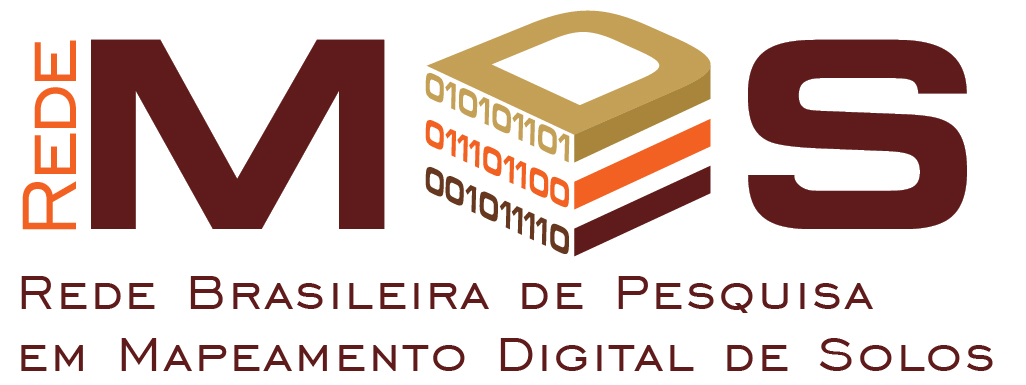
\includegraphics[width=0.8\linewidth]{figuras/redemds}\\
		\caption{\footnotesize \textbf{Rede Brasileira de Pesquisa em Mapeamento Digital de Solos.}}
	\end{center}
	
	Durante a Segunda Reunião da Rede Brasileira de Pesquisa em Mapeamento Digital de Solos (RedeMDS), realizada em outubro de 2012 na cidade de Florianópolis, SC, os cursos de capacitação por EaD foram amplamente debatidos e aprovados. Precisamos, com urgência, por em práticas esses cursos de capacitação através dessa modalidade, onde poderíamos, através das tecnologias disponíveis (Moodle, por exemplo), capacitar um público ávido por informações de pedologia (novos professores, pesquisadores, extensionistas, estudantes de pós-graduação, entre outros) que, por dificuldades de deslocamento a grandes centros e mesmo pela falta de cursos, se desinteressam ou não se interessam pela pedologia. A Sociedade Brasileira de Ciência do Solo, ciente do potencial do EaD, discutirá, através do simpósio número 8, durante o XXXIV Congresso Brasileiro de Ciência do Solo, a Educação à distância em solos. Será um interessante espaço de debates e quiça, antes mesmo da realização do XXXIV CBCS que inicia no dia 28 de Julho em Florianópolis, o grupo que compõe a RedeMDS possa oferecer, mesmo que em regime de “experiência”, uma capacitação em pedologia, abordando claro, MDS. É minha opinião. Aliás, meu desejo, e espero que o mesmo se concretize, pois também faço parte do grupo idealizador dessa proposta.\par}
	
	\begin{center}
		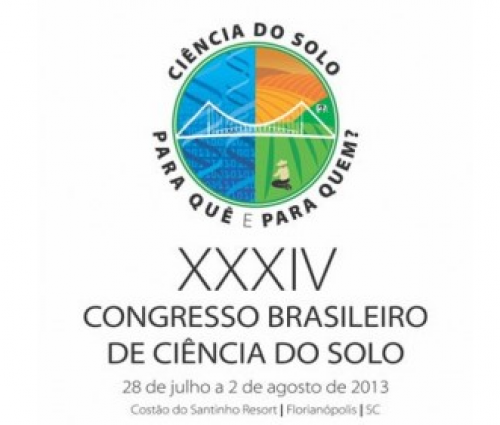
\includegraphics[width=0.8\linewidth]{figuras/cbcs}\\
		\caption{\footnotesize \textbf{XXXIV Congresso Brasileiro de Ciência do Solo.\\Fonte: SBCS.}}
	\end{center}

	\vspace{0.5cm}
	
	\noindent \textbf{Referências}\\
	\\
	{\footnotesize \noindent Basher, L.R. Is pedology dead and buried? Australian Journal of Soil Research, 35:979-994, 1997.\par}
	{\footnotesize \noindent Dalmolin, R.S.D. Faltam pedólogos no Brasil. Boletim Informativo da Sociedade Brasileira de Ciência do Solo, 24:13-15, 1999.\par}
	{\footnotesize \noindent KER, J. C. O futuro da pedologia no Brasil. Boletim Informativo da Sociedade Brasileira de Ciência do Solo, 24:18-21, 1999.\par}
	\vspace{0.5cm}
	{\footnotesize \noindent \emph{*Ricardo Simão Diniz Dalmolin é professor do Departamento de Solos e coordenador da Universidade Aberta do Brasil na Universidade Federal de Santa Maria.}\par}

\newpage

% -------------------------------------------------------
% Texto sobre o conteúdo pedométrico no XXXIV CBCS
% -------------------------------------------------------
\NewsItem{A Pedometria no XXXIV CBCS}
\NewsAuthor{Alexandre ten Caten}
\begin{wrapfigure}{l}{0.15\textwidth}
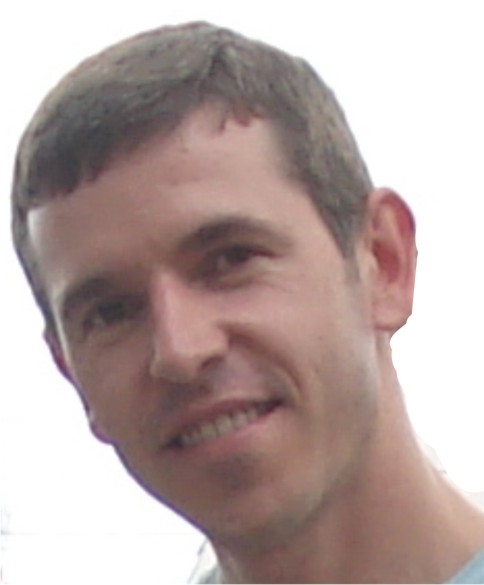
\includegraphics[width=0.15\textwidth]{figuras/ten-caten.jpg}
\end{wrapfigure}
	{\small O XXXIV \href{http://www.cbcs2013.com.br}{Congresso Brasileiro de Ciência do Solo}, a ser realizado entre os dias 28 de julho e 02 de agosto de 2013, está com uma programação recheada de discussões sobre pedometria. O Simpósio \emph{Pedometria: Mitos e fatos}, a ser realizado na manhã do dia 31/07, terá duas palestras. A Palestra 1, intitulada \emph{Pedometria: Histórico, motivações e propósitos}, terá como palestrante Alex McBratney, da Universidade de Sydney, Austrália. Alex McBratney  é um dos pesquisadores de maior expressão mundial em mapeamento digital de solos. Sua palestra possibilitará aos ouvintes um apanhado histórico sobre as motivações e propósitos da abordagem quantitativa do mapeamento de classes e propriedades do solo. Alex McBratney também falará do contexto atual e das demandas que necessitam da informação espacial em solos, e de como estas demandas podem ser supridas pelo mapeamento digital em solos.

	\begin{center}
		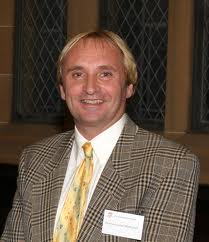
\includegraphics[width=0.8\linewidth]{figuras/mcbratney}\\
		\caption{\footnotesize \textbf{Alex McBratney, da Universidade de Sydney.\\Fonte: sydney.edu.au.}}
	\end{center}
	
	A Palestra 2, intitulada \emph{Interfaces entre o mapeamento convencional e digital de solos}, terá como palestrante Marcos Bacis Ceddia, da Universidade Federal Rural do Rio de Janeiro. Marcos Ceddia irá discutir que o mapeamento de solos necessita de informações (ou dados). Estas informações provêm de levantamentos aerofotogramétricos, de imagens de satélites, de descrições de perfis, de amostras de solos, e de outras tantas fontes. Todas estas distintas fontes de informação são cruciais para que o pedólogo possa definir a distribuição espacial de classes e/ou propriedades de solo, seja utilizando de modelos preditivos ou exclusivamente de seu conhecimento tácito. Uma determinada forma de mapeamento poderá ter características mais qualitativas ou quantitativas, mas poderá ser difícil definir se um determinado levantamento de solos usou exclusivamente de uma abordagem convencional ou digital de mapeamento do solo. Assim, para Marcos Ceddia, as abordagens são complementares.
	
	\begin{center}
		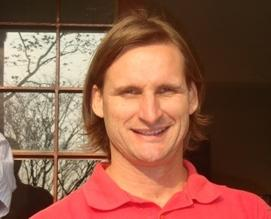
\includegraphics[width=0.8\linewidth]{figuras/bacis}\\
		\caption{\footnotesize \textbf{Marcos Bacis Ceddia, da Universidade Federal Rural do Rio de Janeiro.\\Fonte: www.ia.ufrrj.br.}}
	\end{center}

	O Simpósio \emph{Desafios para o mapeamento digital de solos}, a ser realizado na manhã do dia 01/08, também será composto por duas palestras. A Palestra 1, intitulada \emph{Mapeamento do solo global em um mundo em transformação}, terá como palestrante Sabine Grunwald, da Universidade da Florida. Segundo Sabine Grunwald, os ecossistemas têm sido submetidos a mudanças profundas aceleradas em todo o mundo, o que impõe ameaças para o funcionamento e a sustentabilidade da produção agrícola e dos sistemas naturais. Alterações globais, tais como o crescimento populacional, a mudança climática, e alterações drásticas do uso da terra, impõe marcas profundas no ecossistema solo que impactam a qualidade do solo, as funções do solo, a biodiversidade e a segurança alimentar. A avaliação da distribuição,  padrões e evolução das propriedades do solo em escala global sob tais pressões impostas pela mudança global apresenta novos desafios. Mapas de solo, modelos e abordagens digitais permitem sintetizar o conhecimento em prol do mapeamento mundial do solo em um mundo em mudança. Durante sua fala, Sabine Grunwald discutirá as abordagens de mapeamento digital de solos contemporâneos, além de apresentar uma visão para o futuro do mapeamento e modelagem digital de solos.
	
	\begin{center}
		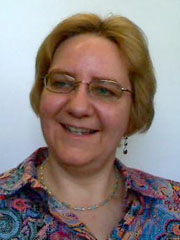
\includegraphics[width=0.8\linewidth]{figuras/sabine}\\
		\caption{\footnotesize \textbf{Sabine Grunwald, da Universidade da Florida.\\Fonte: www.ufl.edu.}}
	\end{center}
	
	A Palestra 2, intitulada \emph{Retrospectiva e desafios para o mapeamento digital de solos no Brasil}, terá como palestrante Maria de Lourdes Mendonça Santos Brefin, da Embrapa Solos. Segundo Maria de Lourdes, desde de 2006, por ocasião do 2° Workshop Global em Mapeamento Digital de Solos realizado no Rio de Janeiro, os pesquisadores brasileiros têm tido um contato maior com a abordagem quantitativa para o mapeamento de classes e propriedades de solos. Em sua palestra, a pesquisadora traçará uma retrospectiva dos avanços experimentados pelo mapeamento digital de solos realizado no país, assim como indicará alguns desafios a enfrentar. Questões como a continentalidade do país, os grandes vazios de levantamentos de solos e a falta de uniformidade nos métodos laboratoriais, precisam ser abordados na medida em que se propõem o desenvolvimento de uma metodologia nacional de mapeamento de propriedades de solos através da RedeMDS (Rede brasileira de Mapeamento Digital de Solos).
	
	\begin{center}
		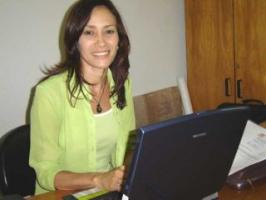
\includegraphics[width=0.8\linewidth]{figuras/lou}\\
		\caption{\footnotesize \textbf{Maria de Lourdes Mendonça Santos Brefin, da Embrapa Solos.\\Fonte: www.embrapa.br.}}
	\end{center}
	\par}
	
	
	\vspace{0.5cm}
	{\footnotesize \noindent \emph{*Alexandre ten Caten é professor Adjunto na Universidade Federal de Santa Catarina campus Curitibanos.}\par}
	
\newpage
% -------
% Eventos
% -------
\NewsItem{Eventos}
\NewsAuthor{Vasily Dokuchaev}
\begin{wrapfigure}{l}{0.15\textwidth}
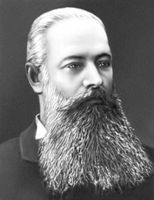
\includegraphics[width=0.15\textwidth]{figuras/dokuchaev.jpg}
\end{wrapfigure}
	{\small Diversos eventos serão realizados durante os próximos meses, nos quais a pedometria já tem, ou pode vir a ter, papel de destaque. Alguns serão realizados no Brasil, como o Congresso Brasileiro de Ciência do Solo. Mas a maioria ocorre no exterior. Veja abaixo a lista de eventos que selecionei:
	
	\begin{itemize}
	 \item 3 a 6 de junho de 2013. IUSS Global Soil Carbon Conference. Madison, EUA. \url{http://iuss-c-conference.org}
	 
	 \item 28 de julho a 2 de agosto de 2013. Congresso Brasileiro de Ciência do Solo. Florianópolis, Brasil. \url{http://www.eventossolos.org.br/cbcs2013/}
	 
	 \item 4 a 6 de setembro de 2013. Conferência da Comissão 3.6 da IUSS. Utilization and protection of halophytes and salt-affected landscapes. Kecskemét, Hungria. \url{http://members.iif.hu/tot3700/salinityconferencehungary2013.html}
	 
	 \item 30 de setembro a 5 de outubro de 2013. Soils in Space and Time. Conferência da Divisão 1 da IUSS. Ulm, Alemanha. \url{https://iuss-division1.uni-hohenheim.de}
	 
	 \item 7 a 9 de outubro de 2013. Encontro do Grupo de Trabalho GlobalSoilMap da IUSS. Orleans, Françe. \url{https://colloque.inra.fr/globalsoilmap2013}
	 
	 \item 16 a 20 de outubro de 2013. Geomorphometry 2013. Nanjing, China. \url{http://geomorphometry.org/category/keywords/conference}
	 
	 \item 26 a 28 de março de 2014. Soil Change Matters. Encontro combinado dos Grupos de Trabalho da IUSS em Mudança do Solo, Monitoramento do Solo e Sensoriamento Proximal do Solo. Bendigo, Austrália. Entre em contato com \href{mailto:Richard.MacEwan@dpi.vic.gov.au}{Richard.MacEwan@dpi.vic.gov.au} para maiores informações.
	\end{itemize}
	\par}
\end{multicols}

\vspace{0.5cm}
\SepRule
\vspace{0.5cm}

\begin{multicols}{3}
\NewsItem{Informações Gerais}
{\small Esse documento foi elaborado utilizando o modelo desenvolvido e disponibilizado gratuitamente pela equipe do site \url{http://www.howtotex.com}. Para entrar em contato com os autores, envie mensagem para o endereço de e-mail \href{mailto:frits@howtotex.com}{frits@howtotex.com}

Para enviar artigo, sugestão, reclamação ou solicitar qualquer informação sobre a Newsletter da Comissão de Pedometria da SBCS, envie mensagem para o endereço de e-mail \href{mailto:alessandrosamuel@yahoo.com.br}{alessandrosamuel@yahoo.com.br} ou \href{mailto:bueno.jean1@gmail.com}{bueno.jean1@gmail.com}.

Os textos enviados para publicação na Newsletter da Comissão de Pedometria da SBCS devem ser redigidos em língua portuguesa, preferencialmente com voz ativa e linguagem informal. Os textos devem ter o tamanho de aproximadamente 1 página no formato A4, redigidos com fonte Times New Roman, tamanho 12, espaçamento um e meio, com margens de 2,5 cm. Os documentos devem ser enviados no formato *.doc, *.odf, *.txt ou *.tex. A correção ortográfica e gramatical é de responsabilidade do autor.\par}
\end{multicols}
  
% ----- Final do documento
\end{document} 

